\documentclass[11pt]{article}

\usepackage[margin=1in]{geometry}
\usepackage{booktabs}
\usepackage{array}
\usepackage{longtable}
\usepackage{hyperref}
\usepackage{xcolor}
\usepackage{tikz}
\usepackage{amsmath}
\usepackage{fancyhdr}
\usepackage{caption}
\usetikzlibrary{arrows.meta,positioning,shapes.geometric,fit,calc}

\hypersetup{
  colorlinks=true,
  linkcolor=blue!60!black,
  urlcolor=blue!60!black,
  citecolor=blue!60!black
}

\pagestyle{fancy}
\setlength{\headheight}{14pt}
\fancyhf{}
\lhead{DLR-Lambda Loghub Experiment}
\rhead{Nikit Phadke}
\cfoot{\thepage}

\newcommand{\code}[1]{\texttt{\detokenize{#1}}}
\newcommand{\pass}{\textsc{pass}}
\newcommand{\fail}{\textsc{fail}}
\newcolumntype{L}[1]{>{\raggedright\arraybackslash}p{#1}}
\setlength{\emergencystretch}{2em}

\title{\textbf{Recursive Log Diagnosis with ProcessIR:}\\
A DLR-Lambda Experiment on Loghub}
\author{Nikit Phadke}
\date{June 2026}

\begin{document}
\maketitle

\begin{abstract}
Operational logs often contain a failure's causal evidence, but the evidence is
rarely adjacent, self-contained, or expressed as an explicit root cause. A local
subsystem may report success while the parent process has not reached a valid
terminal state. This paper reports a standalone experiment combining a
lambda-style recursive execution plan, inspired by lambda-RLM \cite{lambda_rlm},
with Disentangled Language Representation (DLR) ProcessIR diagnosis. The
experiment uses the public Loghub Linux log
sample as a real noisy substrate and injects five distant synthetic evidence
events that encode a stale-policy failure. A direct first-window parser fails to
recover the incident. A naive chunk event merge recovers the observed events but
misses the latent stale-representation root cause. The DLR-lambda pipeline,
implemented as deterministic split, map, filter, and reduce stages, recovers all
event nodes, the latent condition, all causal edges, the root cause, the false
terminal state, and a corrective prescription. The result is not presented as a
general benchmark score. It is a falsification-style demonstration that typed
recursive control and typed causal intermediate representations solve different
parts of the log diagnosis problem: recursion makes distributed evidence
tractable, while ProcessIR makes the reduced result semantically inspectable.
\end{abstract}

\section{Introduction}

Many incident traces are not failures of a single action. They are failures of
composition. One component reports a local terminal state, while another
component later reveals that the parent workflow was never globally complete.
This pattern is common in release pipelines, account workflows, payments,
compliance processes, and agentic tool-use systems. A logging system may
therefore contain all required evidence while still making the incident hard to
diagnose: the relevant lines are separated by noise, time, service boundaries,
and representation boundaries.

The experiment in this paper asks a narrow question:

\begin{quote}
Can a recursive, lambda-style execution plan recover a typed DLR ProcessIR
diagnosis from distributed evidence embedded in realistic logs?
\end{quote}

The implemented answer is yes for the constructed probe. The result is valuable
because it separates two problems that are often collapsed. Lambda-RLM argues
that typed symbolic control can make long-context recursive reasoning more
verifiable and efficient than open-ended recursive code generation
\cite{lambda_rlm}. This experiment asks what typed recursive control should
compose \emph{into} for incident diagnosis. First, there is a
\emph{control problem}: how to scan and compose evidence across a long sequence
without assuming it is adjacent. Second, there is a \emph{semantic target
problem}: what structure should the diagnosis produce once the evidence is
found? The proposed pipeline addresses the first problem with typed recursive
operators and the second with ProcessIR.

The contribution is an executable micro-benchmark over Loghub Linux logs
\cite{loghub_repo,loghub_issre,loghub2_issta} that combines lambda-RLM-style
recursive control with a DLR ProcessIR target. The benchmark includes three
systems: a direct first-window parser, a naive chunk event merge, and the
DLR-lambda ProcessIR reducer. Only the third system recovers the latent root
cause and the full causal graph.

\section{Background}

\subsection{Lambda-RLM}

Lambda-RLM replaces free-form recursive control code with a typed functional
runtime grounded in lambda calculus \cite{lambda_rlm}. In that setting,
recursive reasoning is expressed through a compact library of verified
combinators, and neural inference is applied to bounded leaf subproblems. This
paper does not reimplement the full lambda-RLM system. It borrows the core
control idea: make long-context reasoning a typed recursive program rather than
an unstructured prompt over an entire context.

The difference is the output target. Lambda-RLM primarily addresses reliable
long-context control. DLR ProcessIR addresses typed semantic diagnosis. The
experiment tests their combination: recursive control over log chunks, followed
by reduction into a causal process graph.

\subsection{Loghub as Noisy Substrate}

Loghub is a public collection of system log datasets for AI-driven log analytics
research \cite{loghub_repo,loghub_issre}. Its repository describes datasets
from distributed systems, operating systems, mobile systems, server
applications, and standalone software. The experiment uses the Linux log sample,
which is small enough to download and run locally while still providing a real
background of unstructured operating-system log lines.

The benchmark does not claim that the original Loghub Linux sample contains the
target incident. Instead, it uses Loghub as the noisy carrier and injects a
controlled synthetic incident. This lets the experiment keep a known gold graph
while testing whether the parser can recover evidence distributed across a real
log stream.

\subsection{ProcessIR}

ProcessIR is the process-level intermediate representation used by the DLR
experiments. The relevant fields for this paper are:

\begin{itemize}
  \item \textbf{event frames}: observed events with roles such as
  false-terminal state, invariant violation, and terminal outcome;
  \item \textbf{latent conditions}: inferred structural causes that are not
  themselves single log events;
  \item \textbf{causal graph}: typed edges between event frames and latent
  conditions;
  \item \textbf{diagnosis}: motif-level explanation of the failure;
  \item \textbf{prescription}: corrective action at the motif level;
  \item \textbf{confidence}: calibrated confidence for the diagnosis.
\end{itemize}

The key semantic distinction is local versus global completion. A local
transition can be successful and still be globally invalid if it violates a
parent invariant or is based on a stale representation.

\section{Experimental Design}

\subsection{Incident Construction}

The experiment injects five evidence lines into \code{Linux_2k.log}. The final
trace has 2005 lines. Evidence is intentionally separated across chunks so that
a single-window parser cannot see the incident and a shallow event merge lacks
the pressure to infer the hidden precondition.

\begin{table}[h]
\centering
\caption{Injected distributed evidence.}
\small
\begin{tabular}{r p{0.78\linewidth}}
\toprule
Line & Evidence summary \\
\midrule
121 & Policy cache has a long TTL and is treated as the local policy source. \\
482 & Authoritative policy changes to version v18 and now requires manager review. \\
953 & Worker reports local success and approves refund R-913 using cached policy v17. \\
1304 & Audit detects invariant violation: expected v18, observed v17, manager review missing. \\
1705 & Finance blocks settlement because the approval was not a valid terminal state. \\
\bottomrule
\end{tabular}
\end{table}

The gold root cause is not any single event. It is the latent condition:
\emph{the worker approved a refund using stale cached policy v17 after the
authoritative policy changed to v18}. This is a representation and decay failure
that produces a false terminal state.

\subsection{Recursive Execution Plan}

The DLR-lambda execution plan is deliberately simple:

\begin{verbatim}
SPLIT(log_lines, chunk_size=350)
MAP(parse_chunk_to_event_frames)
FILTER(relevant_incident_frames)
REDUCE(infer_latent_conditions + merge_causal_graph)
OUTPUT(ProcessIR + prescription)
\end{verbatim}

The important operation is the reduce step. The reduce stage composes local
evidence into a latent condition and typed causal graph. It is therefore not
merely concatenating parsed events.

\begin{figure}[h]
\centering
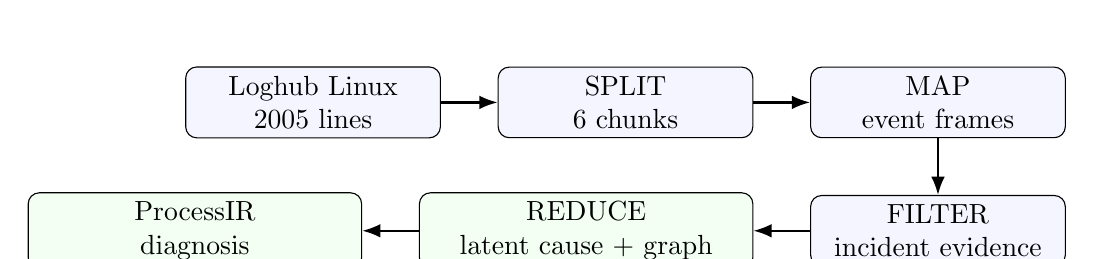
\begin{tikzpicture}[
  node distance=0.72cm,
  box/.style={draw, rounded corners, align=center, minimum height=0.78cm,
    text width=3.0cm, fill=blue!4},
  wide/.style={draw, rounded corners, align=center, minimum height=0.78cm,
    text width=4.0cm, fill=green!5},
  arr/.style={-Latex, thick}
]
\node[box] (logs) {Loghub Linux\\2005 lines};
\node[box, right=of logs] (split) {SPLIT\\6 chunks};
\node[box, right=of split] (map) {MAP\\event frames};
\node[box, below=of map] (filter) {FILTER\\incident evidence};
\node[wide, left=of filter] (reduce) {REDUCE\\latent cause + graph};
\node[wide, left=of reduce] (out) {ProcessIR\\diagnosis};
\draw[arr] (logs) -- (split);
\draw[arr] (split) -- (map);
\draw[arr] (map) -- (filter);
\draw[arr] (filter) -- (reduce);
\draw[arr] (reduce) -- (out);
\end{tikzpicture}
\caption{DLR-lambda execution plan. Recursive control finds distributed evidence;
ProcessIR gives the reduction a typed semantic target.}
\end{figure}

\subsection{Systems Compared}

The benchmark compares three systems:

\begin{enumerate}
  \item \textbf{Direct first-window parser}: runs a DLR-style parser on the
  first chunk only. This tests what happens when the diagnosis has access to
  local context but not the distributed trace.
  \item \textbf{Naive chunk event merge}: parses all chunks and merges observed
  event frames, but does not infer latent conditions during reduction.
  \item \textbf{DLR-lambda ProcessIR}: parses chunks, filters incident evidence,
  and reduces evidence into latent conditions, causal edges, root cause, and
  prescription.
\end{enumerate}

\section{Gold ProcessIR}

The gold graph contains three observed event nodes, one latent condition, and
three typed causal edges.

\begin{figure}[h]
\centering
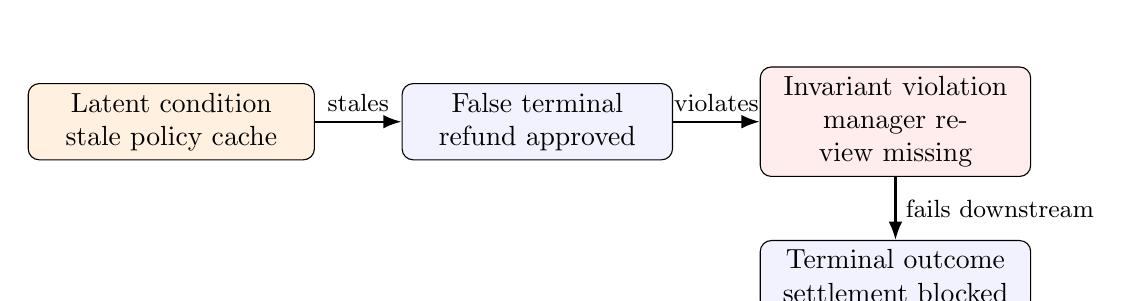
\begin{tikzpicture}[
  node distance=0.8cm and 1.1cm,
  latent/.style={draw, rounded corners, align=center, fill=orange!12,
    text width=3.4cm, minimum height=0.9cm},
  event/.style={draw, rounded corners, align=center, fill=blue!5,
    text width=3.2cm, minimum height=0.9cm},
  bad/.style={draw, rounded corners, align=center, fill=red!7,
    text width=3.2cm, minimum height=0.9cm},
  arr/.style={-Latex, thick}
]
\node[latent] (latent) {Latent condition\\stale policy cache};
\node[event, right=of latent] (false) {False terminal\\refund approved};
\node[bad, right=of false] (inv) {Invariant violation\\manager review missing};
\node[event, below=of inv] (term) {Terminal outcome\\settlement blocked};
\draw[arr] (latent) -- node[above, font=\small]{stales} (false);
\draw[arr] (false) -- node[above, font=\small]{violates} (inv);
\draw[arr] (inv) -- node[right, font=\small]{fails downstream} (term);
\end{tikzpicture}
\caption{Gold causal graph for the injected incident.}
\end{figure}

\section{Results}

\begin{table}[h]
\centering
\caption{System-level scores.}
\small
\begin{tabular}{lrrrrrccc}
\toprule
System & Conf. & Event & Latent & Edge & Root & False & L/G & Result \\
 & & recall & recall & recall & cause & terminal & sep. & \\
\midrule
Direct first-window parser & 0.86 & 0.00 & 0.00 & 0.00 & 0.00 & no & no & \fail \\
Naive chunk event merge & 0.78 & 1.00 & 0.00 & 0.67 & 0.00 & yes & yes & \fail \\
DLR-lambda ProcessIR & 0.86 & 1.00 & 1.00 & 1.00 & 1.00 & yes & yes & \pass \\
\bottomrule
\end{tabular}
\end{table}

\begin{figure}[h]
\centering
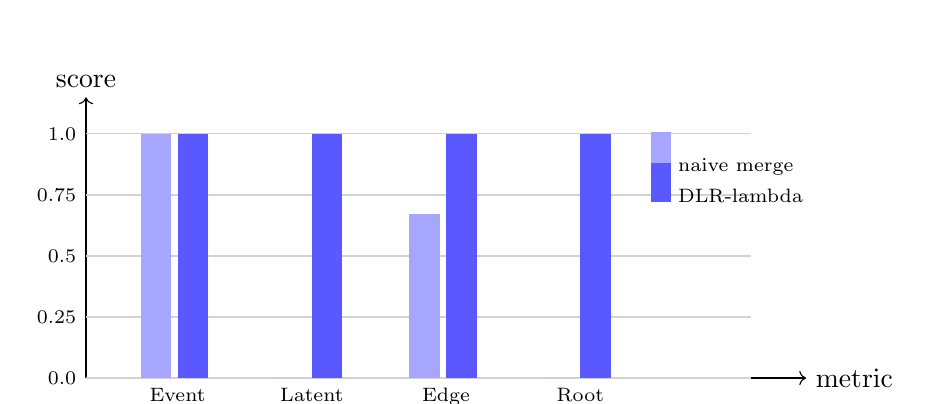
\begin{tikzpicture}[x=1.55cm,y=3.1cm]
  \draw[->] (0,0) -- (5.9,0) node[right] {metric};
  \draw[->] (0,0) -- (0,1.15) node[above] {score};
  \foreach \y/\lab in {0/0.0,0.25/0.25,0.5/0.5,0.75/0.75,1/1.0} {
    \draw[gray!35] (0,\y) -- (5.45,\y);
    \node[left,font=\scriptsize] at (0,\y) {\lab};
  }
  \foreach \x/\lab in {0.75/Event,1.85/Latent,2.95/Edge,4.05/Root} {
    \node[below,font=\scriptsize,align=center] at (\x,0) {\lab};
  }
  \fill[blue!35] (0.45,0) rectangle (0.70,1.00);
  \fill[blue!65] (0.75,0) rectangle (1.00,1.00);
  \fill[blue!35] (1.55,0) rectangle (1.80,0.00);
  \fill[blue!65] (1.85,0) rectangle (2.10,1.00);
  \fill[blue!35] (2.65,0) rectangle (2.90,0.67);
  \fill[blue!65] (2.95,0) rectangle (3.20,1.00);
  \fill[blue!35] (3.75,0) rectangle (4.00,0.00);
  \fill[blue!65] (4.05,0) rectangle (4.30,1.00);
  \node[font=\scriptsize,anchor=west] at (4.55,0.92) {\tikz\fill[blue!35] (0,0) rectangle (0.16,0.16); naive merge};
  \node[font=\scriptsize,anchor=west] at (4.55,0.80) {\tikz\fill[blue!65] (0,0) rectangle (0.16,0.16); DLR-lambda};
\end{tikzpicture}
\caption{The naive merge sees observed events but misses the latent root cause.
The DLR-lambda reducer recovers both observed and latent structure.}
\end{figure}

\subsection{Interpretation}

The direct first-window parser fails because it observes only the early
configuration evidence. This is expected. The incident is not locally present in
one chunk.

The naive chunk event merge is more interesting. It sees all observed incident
events, detects the false terminal state, and separates local from global
status. However, it does not infer the latent stale-policy condition. It also
misses the causal edge from stale representation to false terminal approval.
This is the critical failure mode: without a typed reduction step, event recall
can look perfect while root-cause accuracy remains zero.

The DLR-lambda ProcessIR system recovers the latent condition and all causal
edges:

\small
\begin{longtable}{L{0.40\linewidth}L{0.18\linewidth}L{0.30\linewidth}}
\caption{Recovered ProcessIR elements.}\\
\toprule
Element & Type & Meaning \\
\midrule
\endfirsthead
\toprule
Element & Type & Meaning \\
\midrule
\endhead
\code{refund_approved_false_terminal} & Event frame & A worker reports local approval using stale policy v17. \\
\code{manager_review_missing} & Event frame & Audit observes the missing manager-review invariant under policy v18. \\
\code{settlement_blocked} & Event frame & Finance blocks downstream settlement. \\
\code{lc_stale_policy_cache} & Latent condition & The policy cache is stale relative to the authoritative policy source. \\
\code{stales} & Causal edge & The latent stale representation produces the false terminal approval. \\
\code{violates} & Causal edge & The false terminal approval violates the manager-review invariant. \\
\code{fails_downstream} & Causal edge & The invariant violation blocks settlement. \\
\bottomrule
\end{longtable}
\normalsize

\section{Why the Result Matters}

The result is a compact demonstration of synergy. Lambda-style recursion and
DLR ProcessIR are not redundant. They contribute different capabilities:

\begin{itemize}
  \item recursive control makes the evidence search compositional and bounded;
  \item typed event frames preserve local status, global status, roles, and
  invariants;
  \item the reduce step infers hidden structural preconditions from separated
  evidence;
  \item ProcessIR makes the final diagnosis inspectable as a causal graph rather
  than a paragraph of plausible prose.
\end{itemize}

The killer observation is that event recall alone is insufficient. The naive
merge obtains perfect observed-event recall while still failing the diagnosis.
The difference between a log summary and an incident diagnosis is the inferred
latent structure.

\section{Limitations}

This experiment is intentionally small and controlled. The injected evidence
uses explicit \code{DLR_LAMBDA} markers, so the benchmark does not test
open-ended log parsing or natural language extraction. The incident is synthetic,
although it is embedded in a real Loghub Linux log substrate. The parser is
deterministic and schema-specific. It should therefore be read as a
falsification probe for the representation and execution plan, not as a claim of
production-grade incident diagnosis.

The result nevertheless establishes a useful target for a larger evaluation:
remove explicit markers, expand to multiple Loghub datasets, introduce distractor
incidents, use learned parsers for chunk-level extraction, and keep the ProcessIR
graph as the adjudication target.

\section{Conclusion}

The DLR-lambda Loghub experiment shows that recursive execution and typed causal
IR are complementary. Recursive split/map/filter/reduce control finds and
composes distributed evidence. ProcessIR preserves the distinctions that matter
for incident diagnosis: false terminal states, local versus global completion,
latent stale representations, violated invariants, root causes, and corrective
prescriptions.

In the implemented probe, the direct parser fails, the naive event merge sees
events but misses the root cause, and the DLR-lambda reducer recovers the full
causal diagnosis. This is the central result: a system can read all the right log
lines and still fail unless it has an intermediate representation capable of
expressing hidden structural preconditions.

\appendix

\section{Appendix: Minimal DLR Context}

The broader DLR project is not assumed to be published prior work in this
paper. This appendix provides only the context needed to make the standalone
experiment understandable.

DLR decomposes language and traces into motifs, frames, graphs, and process
diagnoses. The ProcessIR fields used in this paper descend from the trace-level
DLR experiments:

\begin{itemize}
  \item \textbf{false terminal state}: a local success report that should not be
  treated as a valid parent-process terminal state;
  \item \textbf{violated invariant}: a constraint required for valid completion;
  \item \textbf{latent condition}: an inferred precondition or structural decay
  source not directly present as one event;
  \item \textbf{local/global separation}: distinction between subsystem status
  and parent-process validity;
  \item \textbf{prescription}: motif-level repair, such as invalidating stale
  representations or adding reconciliation barriers.
\end{itemize}

In this experiment, the relevant motifs are Representation, Invariant,
Reconciliation, Boundary, and Decay. The latent stale policy cache is a
Representation/Decay failure. The missing manager review is an Invariant
failure. The blocked settlement is a Reconciliation and terminal-outcome failure.

\section{Appendix: Reproduction}

The experiment is implemented in the repository as:

\begin{verbatim}
npm run run:dlr-lambda
\end{verbatim}

The command downloads the Loghub Linux sample if needed, injects the synthetic
incident, writes the Markdown report, and writes the ProcessIR JSON artifact.

\begin{thebibliography}{9}

\bibitem{lambda_rlm}
Amartya Roy, Rasul Tutunov, Xiaotong Ji, Matthieu Zimmer, and Haitham
Bou-Ammar.
\newblock The Y-Combinator for LLMs: Solving Long-Context Rot with
$\lambda$-Calculus.
\newblock arXiv:2603.20105v1, 2026.
\newblock \url{https://arxiv.org/abs/2603.20105}.

\bibitem{loghub_repo}
LogPAI.
\newblock Loghub: A large collection of system log datasets for AI-driven log
analytics.
\newblock \url{https://github.com/logpai/loghub}.

\bibitem{loghub_issre}
Jieming Zhu, Shilin He, Pinjia He, Jinyang Liu, and Michael R. Lyu.
\newblock Loghub: A Large Collection of System Log Datasets for AI-driven Log
Analytics.
\newblock IEEE International Symposium on Software Reliability Engineering
(ISSRE), 2023.

\bibitem{loghub2_issta}
Zhihan Jiang, Jinyang Liu, Junjie Huang, Yichen Li, Yintong Huo, Jiazhen Gu,
Zhuangbin Chen, Jieming Zhu, and Michael R. Lyu.
\newblock A Large-scale Evaluation for Log Parsing Techniques: How Far are We?
\newblock ACM SIGSOFT International Symposium on Software Testing and Analysis
(ISSTA), 2024.

\end{thebibliography}

\end{document}
